
\begin{frame}{Context : KoroiBot project}
\vspace*{-0.5cm}
\begin{center}
  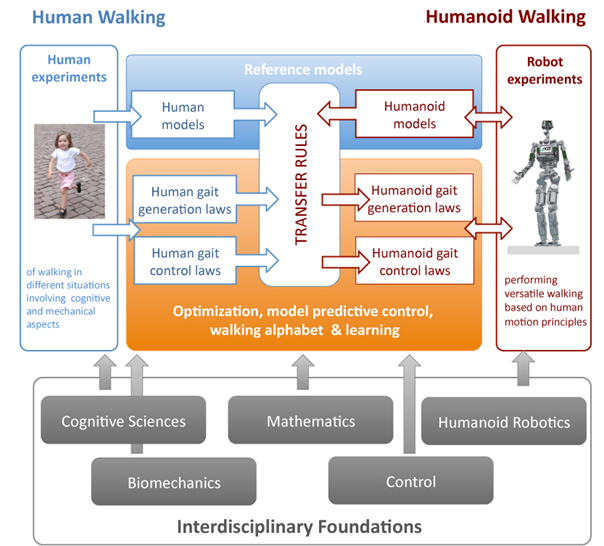
\includegraphics[height=0.7\textheight , keepaspectratio]
  {figures/koroibot/components.png}\\
Goal : enhance the ability of humanoid robots to walk in a dynamic and versatile way, and to bring them closer to human capabilities.
\end{center}
%\begin{itemize}
%  \item 
%\end{itemize}
\end{frame}

\begin{frame}{Context}
\vspace*{-0.7cm}
\begin{columns}
\column{0.6\linewidth}
\begin{center}
  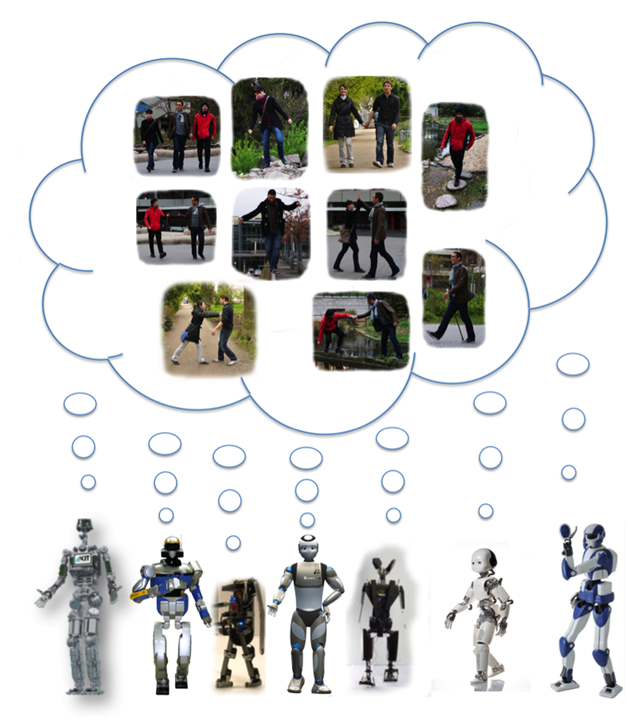
\includegraphics[height=0.9\textheight]{koroibot/situations_v2.png}
\end{center}
\column{0.4\linewidth}
\begin{center}
  
\includegraphics[height=0.1\textheight]{koroibot/logos/cnrs.png}\\
  
\includegraphics[height=0.1\textheight]{koroibot/logos/iit.png}\\
  
\includegraphics[height=0.1\textheight]{koroibot/logos/tud.png}\\
  
\includegraphics[height=0.1\textheight]{koroibot/logos/hd.png}\\
  
\includegraphics[height=0.1\textheight]{koroibot/logos/kit.png}\\
  
\includegraphics[height=0.1\textheight]{koroibot/logos/ut.png}\\
  
\includegraphics[height=0.1\textheight]{koroibot/logos/wi.png}
\end{center}

\end{columns}
%\begin{itemize}
%  \item 
%\end{itemize}
\end{frame}


\begin{frame}{Challenges}
\begin{center}
  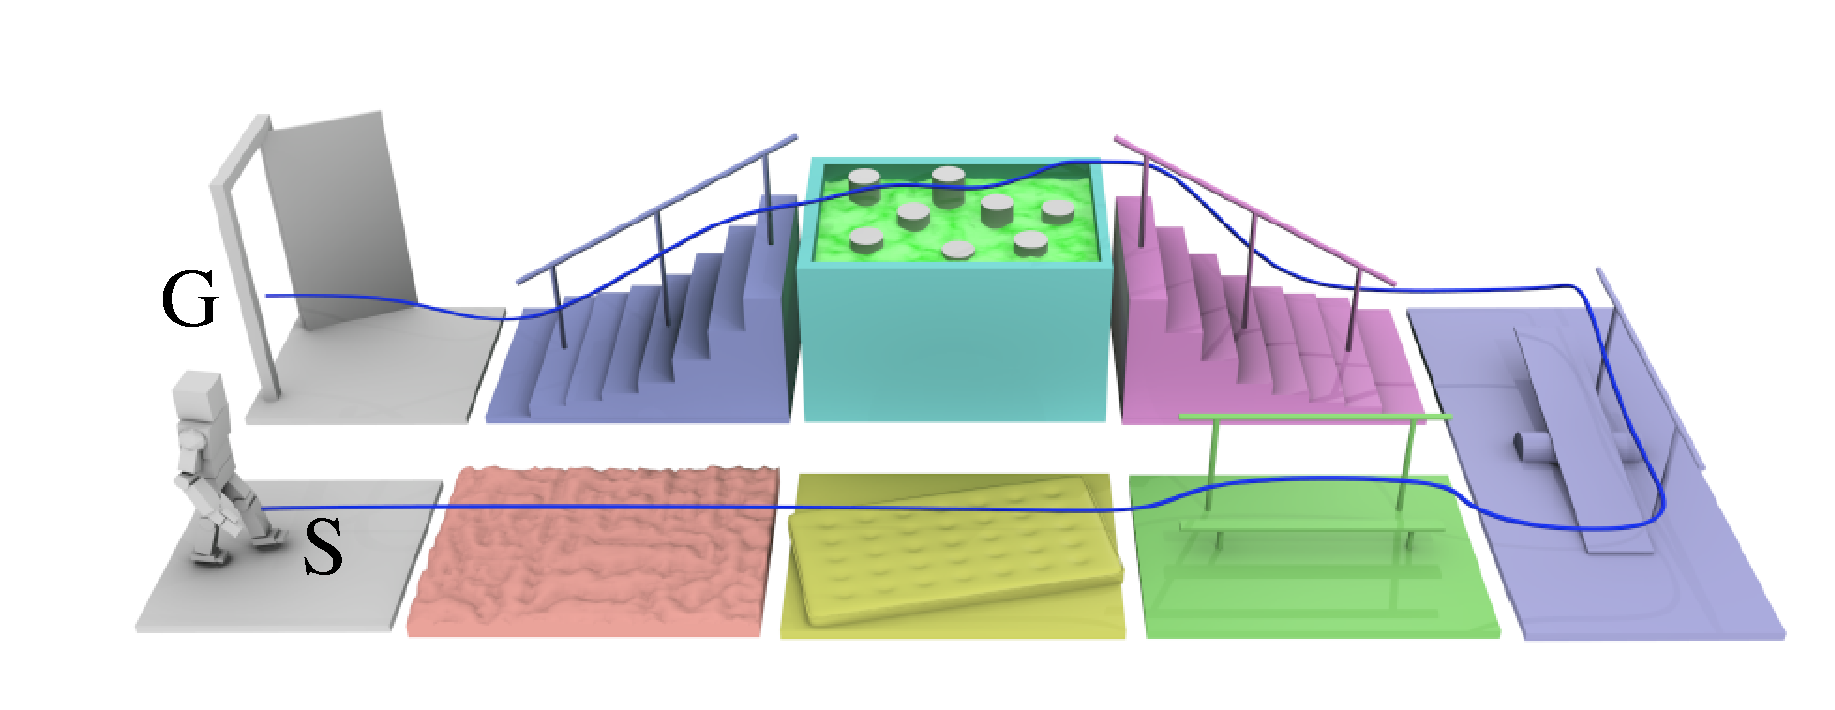
\includegraphics[width=\linewidth]{koroibot/KoroibotChallengeEnhanced.pdf}
  \begin{tikzpicture}[remember picture, overlay]
%    \draw[help lines] (0,0) grid (-1,1);
%    \node at (0,0) {(0,0)};
    \draw[line width=1.5pt, color=red](-10,1) ellipse (0.8cm and .6cm);
    \draw[line width=1.5pt, color=red](-8,1) ellipse (1.1cm and .6cm);
    \draw[line width=1.5pt, color=red](-3.3,1) ellipse (1.1cm and .6cm);
    \draw[line width=1.5pt, color=red](-3.5,3) ellipse (1.0cm and .8cm);
    \draw[line width=1.5pt, color=red](-7.7,3) ellipse (1.0cm and .8cm);
    \draw[line width=1.5pt, color=red](-5.7,3) circle (1.0cm);
  \end{tikzpicture}
\end{center}
%\begin{itemize}
%  \item 
%\end{itemize}
\end{frame}

%
%\begin{frame}{Context}
%\begin{center}
%   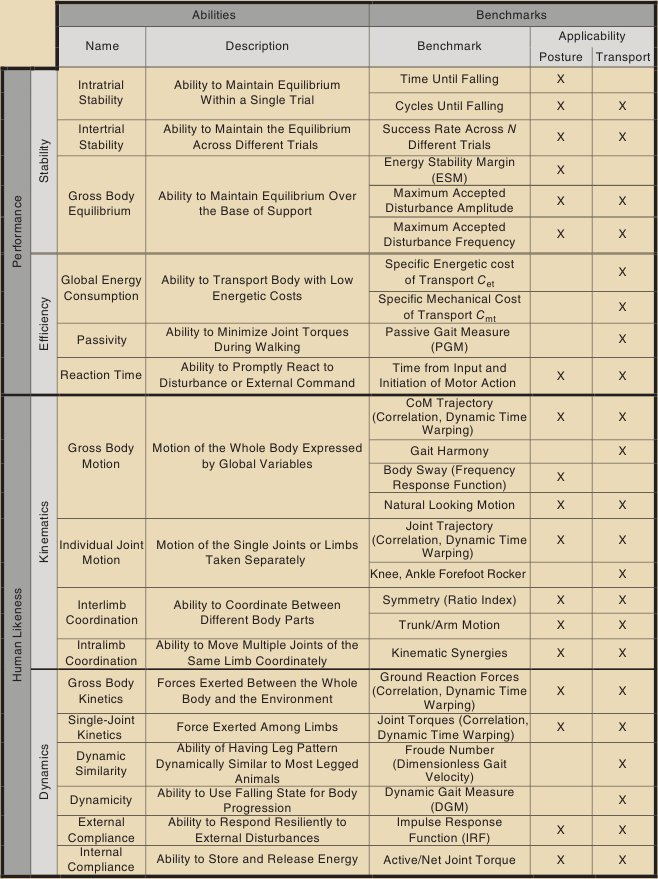
\includegraphics[width=0.90\linewidth]{koroibot/KPIabilities.jpg}
%\begin{tikzpicture}[remember picture, overlay]
%    %\draw[help lines, color=blue] (-8,0) grid (8,25);
%    %\node [color=red] at (0,0) {\textbf (0,0)};
%    %\node [color=red] at (0,20) {\textbf (0,20)};
%    %\node [color=red] at (0,10) {\textbf (0,10)};
%    \draw[line width=1.5pt, color=red](-4.6,16.2) ellipse (2.2cm and .43cm);
%    \draw[line width=1.5pt, color=red](-4.6,13.3) ellipse (2.2cm and .43cm);
%    \draw[line width=1.5pt, color=red](-4.6,12.45) ellipse (2.2cm and .43cm);
%  \end{tikzpicture}
%\end{center}
%%\begin{itemize}
%%  \item 
%%\end{itemize}
%\end{frame}
%
%
%
%\begin{frame}{Context}
%\begin{center}
%   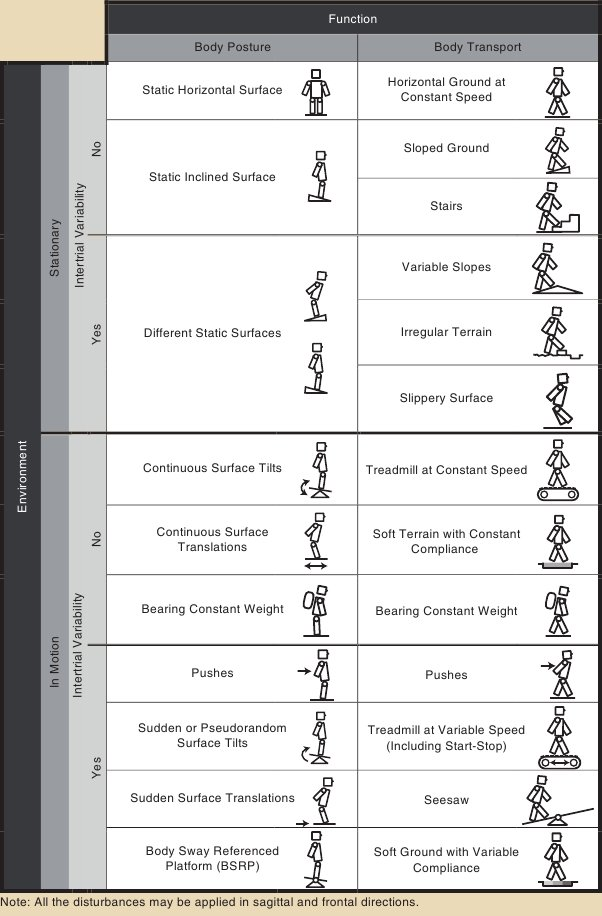
\includegraphics[height=0.9\textheight]{koroibot/KPIexperiment.jpg}
%\begin{tikzpicture}[remember picture, overlay]
%    %\draw[help lines, color=blue] (-8,0) grid (8,25);
%    %\node [color=red] at (0,0) {\textbf (0,0)};
%    %\node [color=red] at (0,20) {\textbf (0,20)};
%    %\node [color=red] at (0,10) {\textbf (0,10)};
%    \draw[line width=1.5pt, color=red](-3.9,19.7) ellipse (2cm and .5cm);
%    \draw[line width=1.5pt, color=red](-3.9,16.9) ellipse (2cm and .5cm);
%    \draw[line width=1.5pt, color=red](-3.9,9.0) ellipse (2cm and .5cm);
%    \draw[line width=1.5pt, color=red](-9.5,7.25) ellipse (2cm and .5cm);
%  \end{tikzpicture}
%\end{center}
%%\begin{itemize}
%%  \item 
%%\end{itemize}
%\end{frame}

\begin{frame}{Problem presentation}

\begin{columns}

\column{0.4\linewidth}

Continuous formulation :

\begin{align*}
\text{min}  &\quad f({\bm q},{\bm v},t) \\
\text{s.t.} &\quad
g({\bm q},{\bm v},t) < 0 \nonumber \\
&\quad h({\bm q},{\bm v},t) = 0 \nonumber
\end{align*}

\vspace*{2.5cm}


\column{0.4\linewidth}

Discrete formulation :

\begin{align*}
\hspace{-3em}	\underset{\substack{\hspace{0.2em} \underline{\bm x}, \; \underline{\bm u}} }{\min } \ \ \  
	& & \hspace{-3em} {\sum_{s=1}^S} \int_{t_{s}}^{t_{s}+\Delta t_s\hspace{-4em}} \ell_{s} (\bm x, \bm u) \, dt \\
	s.t. & \forall t & \dot{\bm{x}} = dyn(\bm x, \bm u) \\
	&  \forall t& \bm\phi \in \mathcal{K} \\
  &  \forall t& {\bm x} \in \mathcal{B}_x \\ 
  &  \forall t& {\bm u} \in \mathcal{B}_u \\ 
	& & \bm x(0) = \bm x_{0} \\
	& & \bm x(T) \in \mathcal{X}_*
\end{align*}

\end{columns}

\end{frame}


\begin{frame}{Dynamics}

General Rigid Body Dynamics :
\begin{equation*}
\mbf{M}(\mq) \ddot{\mq}  + \mbf{C}(\mq, \mqdot)\mqdot + \mbf{G}(\mq) = \mbf{S}^T \mbf{T} + \sum\limits_{k=1}^{K} \mbf{J}_k^T(\mq)
\begin{bmatrix}
{\bf f}_k \\
\bm{\tau}_k
\end{bmatrix}
\end{equation*}
%
Under-Actuated Dynamics :
\begin{equation*}
  [{\bf \lm} \;\;\;\; {\bf \am}]^T= \mbf{A}_G (\mq) \mqdot = \mbf{M}[0:6,:] \mqdot
\end{equation*}
\begin{small}
\begin{align*}
\dot{\bf \lm} = m \ddot{\mbf{c}} = \sum\limits_{k=1}^{K} \; {^0}R_k \mbf{f}_k + m \mbf{g} 
&\rightarrow
m (\ddot{\mbf{c}}-\mbf{g}) = \sum\limits_{k=1}^{K} \; {^0}R_k \mbf{f}_k
\\
\dot{\bf \am} = \sum\limits_{k=1}^{K} (\mbf{p}_k -\mbf{c}) \times \; {^0}R_k \mbf{f}_k  + \bm{\tau}_k
&\rightarrow
m \mbf{c} \times (\ddot{\mbf{c}}-\mbf{g}) + \dot{\bf \am} = \sum\limits_{k=1}^{K} \mbf{p}_k \times {^0}R_k \mbf{f}_k  + \bm{\tau}_k
\end{align*}
\end{small}

\begin{tikzpicture}[remember picture, overlay]
%  \draw[help lines] (0,0) grid (-1,1);
%  \node at (0,0) {(0,0)};
  \draw [line width=1.5pt, color=txtcolor2] (5.3,0.5) rectangle (11.7,3.2);
\end{tikzpicture}

\end{frame}